\section{Simulations With WCM Z Profile}
\label{ch:ZBunchInSimulation}

\begin{frame}{Simulations With WCM Z Profile}
\begin{itemize}
\item The normalized WCM distribution is stored in a TGraph object 
\item We can
	treat a TGraph as a function via spline interpolation between defined
	points 
\item TGraph::Eval does this out of the box 
\item With TGraph::Eval, we obtain the function-like behavior needed for
	transformations.  
\item \textbf{Caveat:} The numeric integration portion of the code consists of
	172 million iterations - so anything in this loop needs to be heavily
	optimized to avoid impossibly long run-times.  
\item \textbf{Caveat:} When using simpler model for the z-bunch profile,
	simulation takes in total, 35 seconds - this is already getting to be
	long, considering that even with a computing cluster, running over many
	variations of a parameter space can lead to tens of thousands of
	simulation instances.
\end{itemize}
\end{frame}

\begin{frame}{Simple Z Profile Simulation}
For review - we have our old z-profile result for a 1000 micron scan step. Simulating this takes about 35 seconds. 
\begin{figure}
\begin{center}
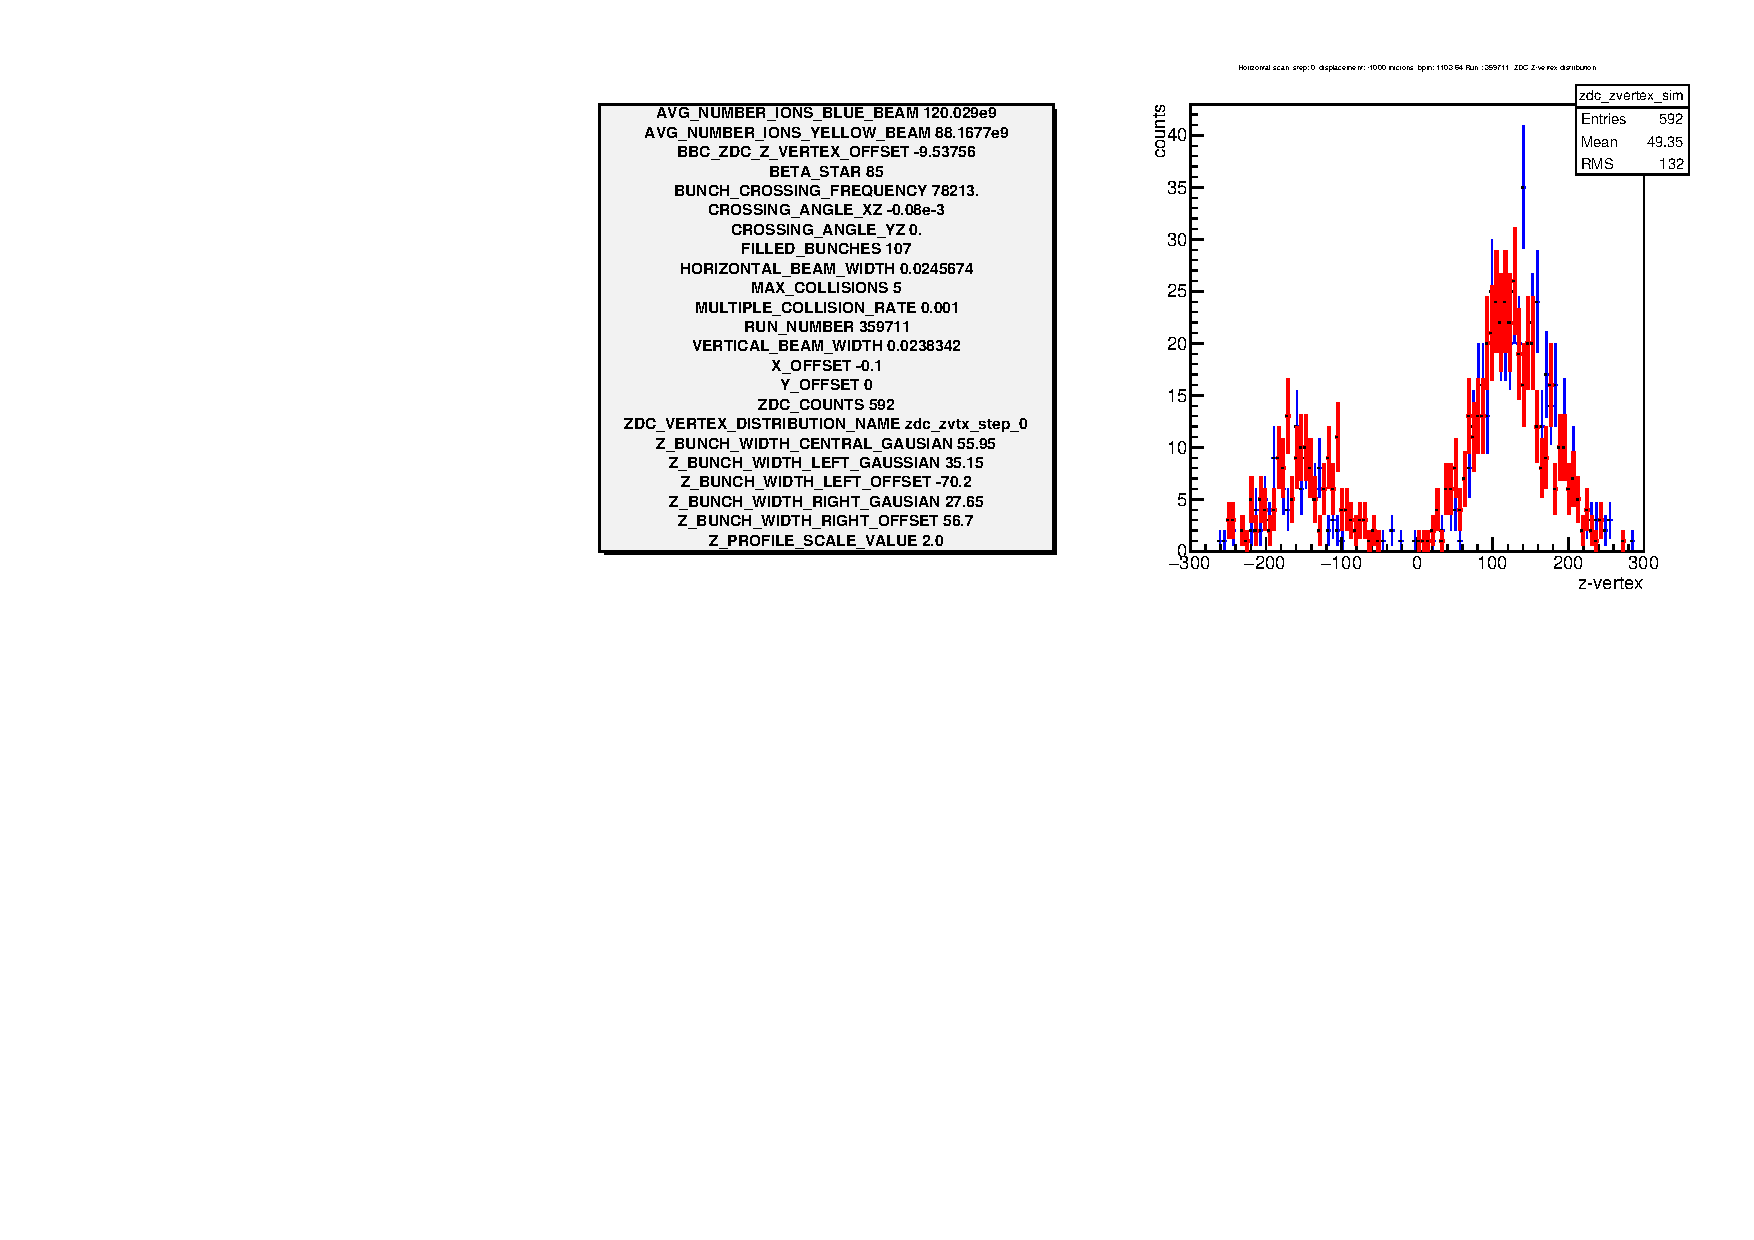
\includegraphics[width=0.75\linewidth]{../ZBunchInSimulation/figs/zvertex_compare_hscan_pos_1000_359711.pdf}
\end{center}
\caption{Using an approximate scaled z-profile for colliding bunches}
\label{fig:zvertex_compare_hscan_pos_1000_359711}
\end{figure}
\end{frame}

\subsection{Real Profile Results, Parmeter Space}
\begin{frame}{Realistic WCM Z Profile Simulation}
Using the exact same simulation configuration as before, we simply replace the
z-profile model with the z bunch profile taken directly from the fine binned
WCM data.
\begin{figure}
\begin{center}
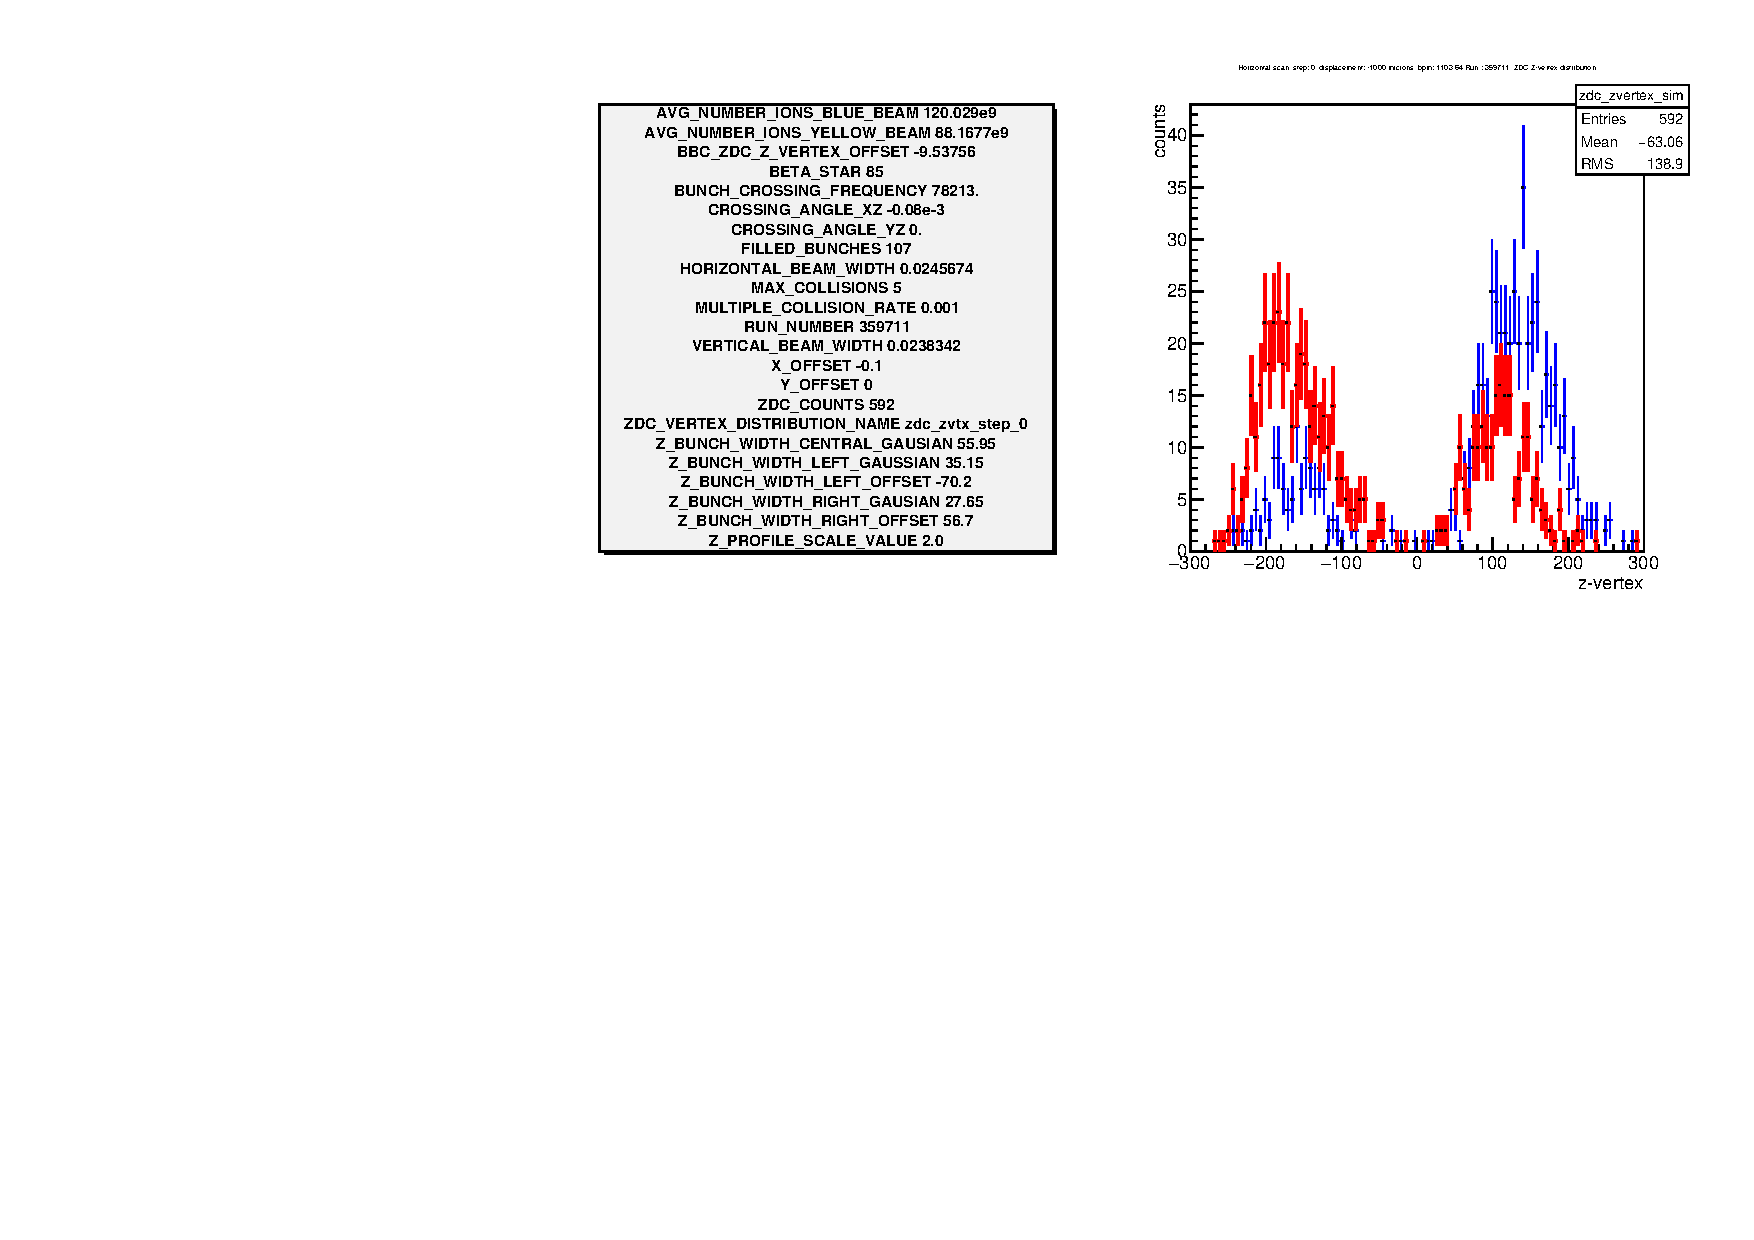
\includegraphics[width=0.75\linewidth]{../ZBunchInSimulation/figs/real_wcm_prof_zvertex_compare_hscan_pos_1000_359711.pdf}
\end{center}
\caption{ Using the "real" Z Profile for colliding bunches}
\label{fig:real_wcm_prof_zvertex_compare_hscan_pos_1000_359711}
\end{figure}
\end{frame}

\begin{frame}{Realistic WCM Z Profile Simulation - Flipped Bunches}
The previous profile looked like it might fit better if it were flipped, since
otherwise the distriubtion implies our crossing angle from
Figure~\ref{fig:zvertex_compare_hscan_pos_1000_359711} is wrong. Here we test if
this affects the z-vertex profile by flipping the bunches.
\begin{figure}
\begin{center}
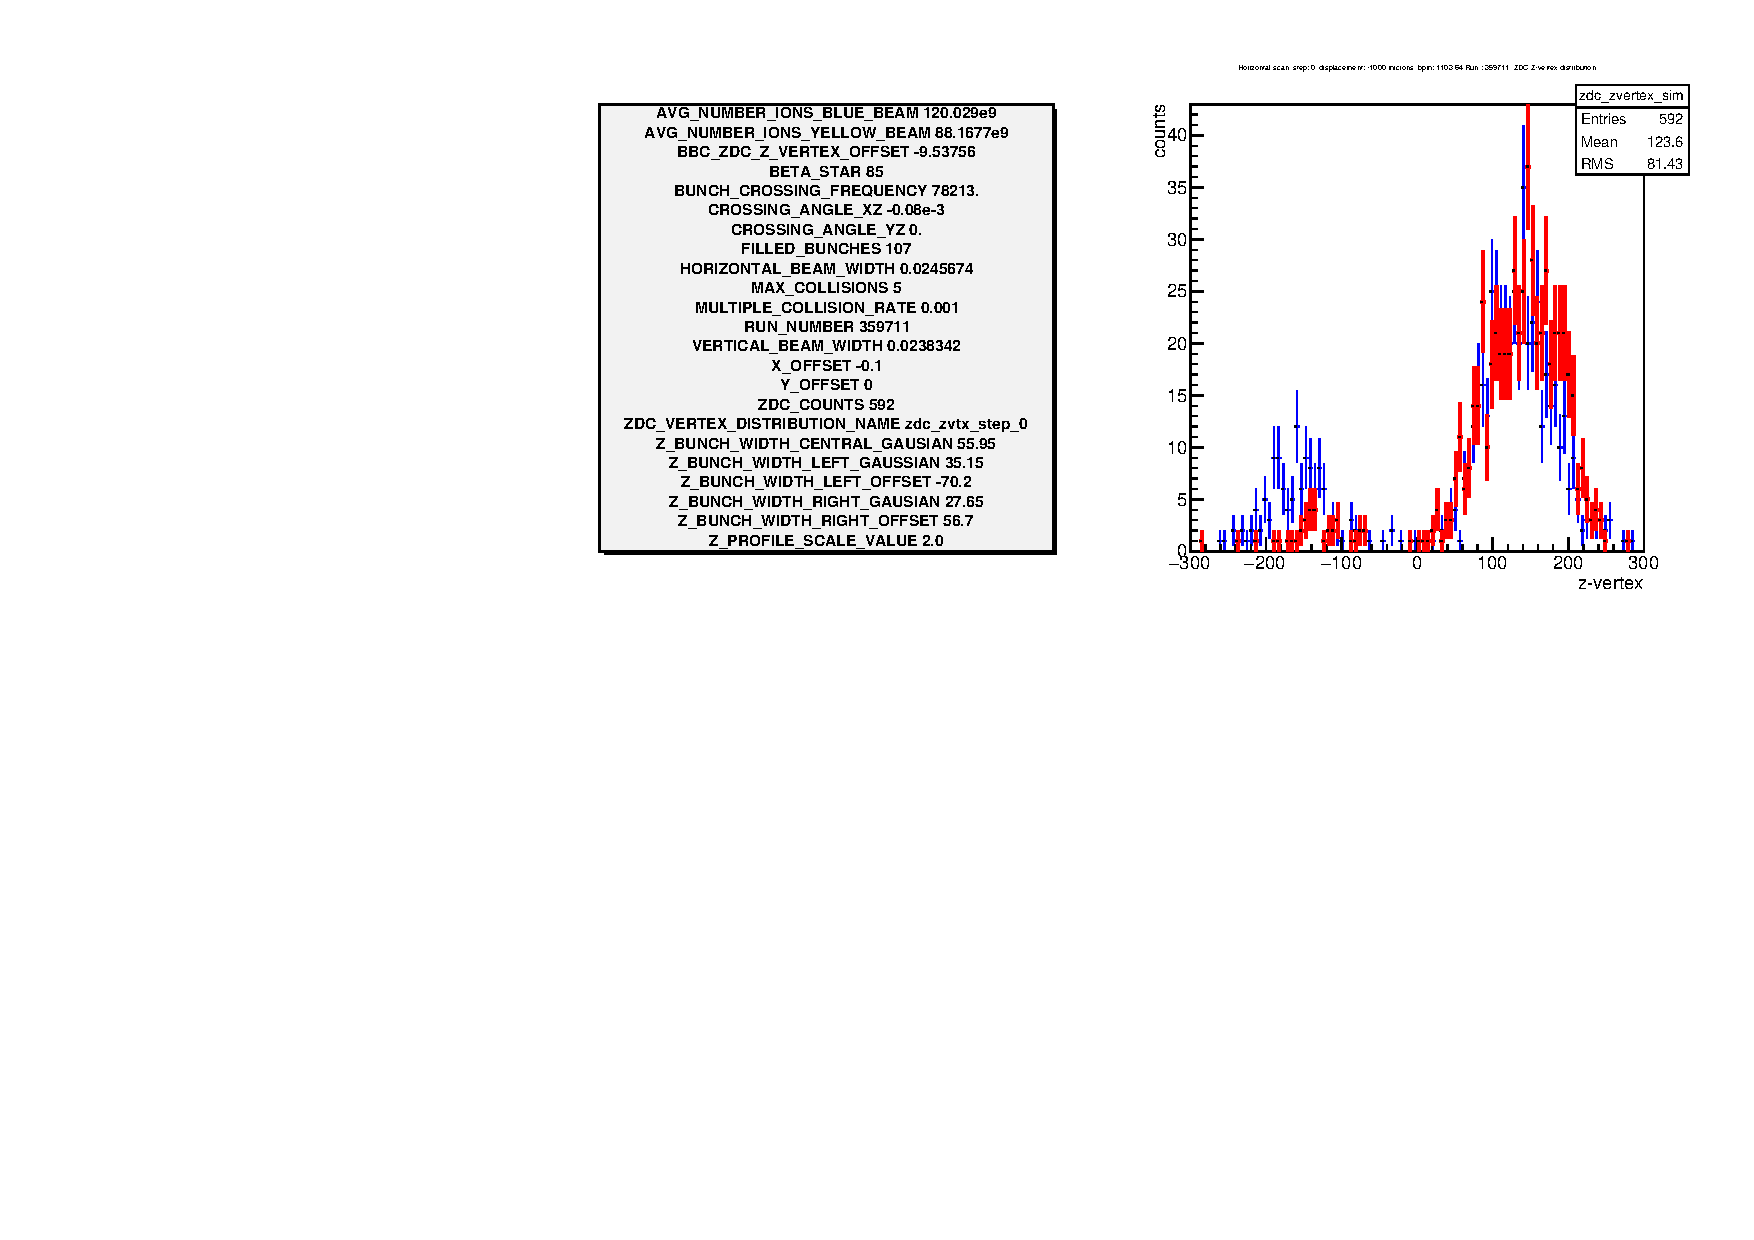
\includegraphics[width=0.75\linewidth]{../ZBunchInSimulation/figs/real_wcm_prof_flipped_zvertex_compare_hscan_pos_1000_359711.pdf}
\end{center}
\caption{ Using the "real" Z Profile for colliding bunches, bunches have been
	flipped along the z-axis}
\label{fig:real_wcm_prof_flipped_zvertex_compare_hscan_pos_1000_359711}
\end{figure}
\end{frame}

\begin{frame}{Realistic WCM Z Profile Simulation - Positive Crossing Angle}
Here, we take the "normal" orientation of the bunches, and collide them with the
opposite sign crossing angle.
\begin{figure}
\begin{center}
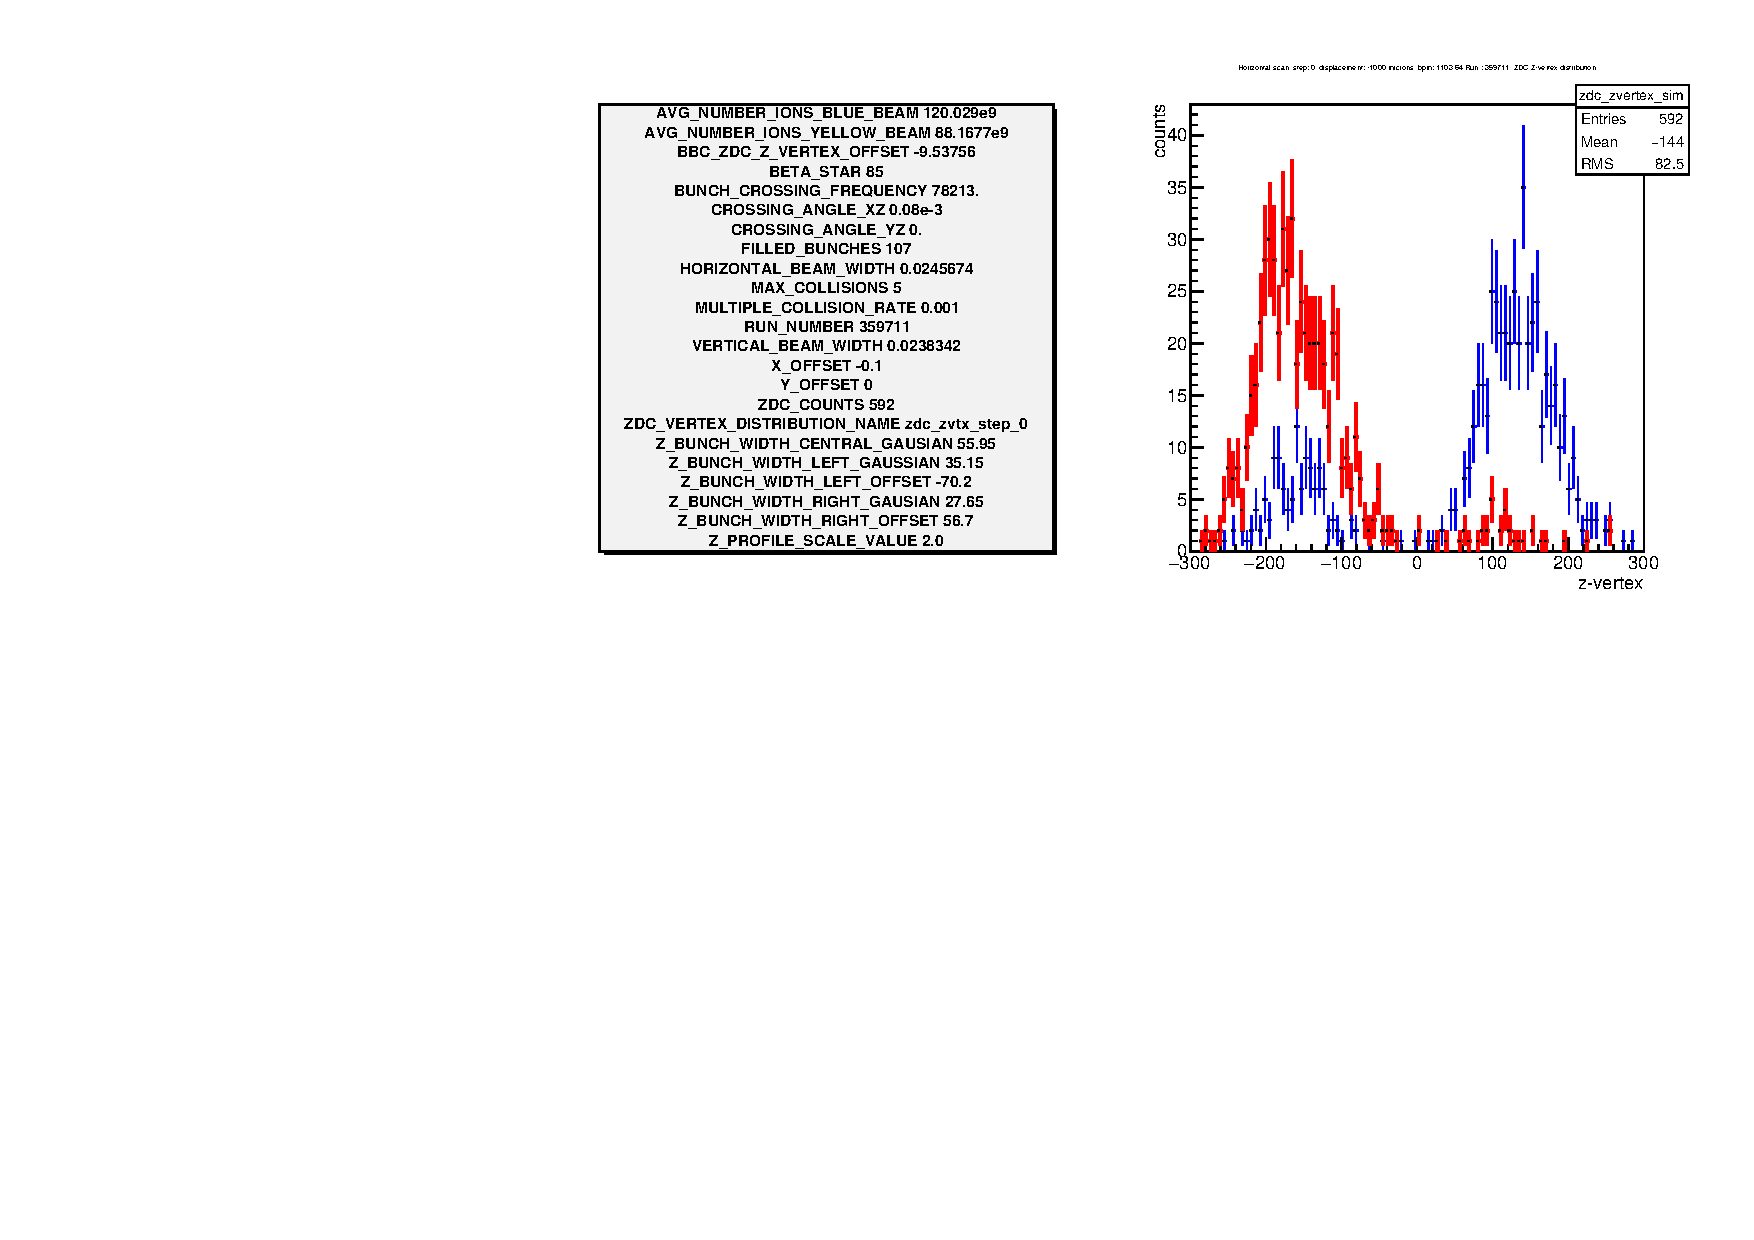
\includegraphics[width=0.75\linewidth]{../ZBunchInSimulation/figs/real_wcm_prof_zvertex_compare_hscan_pos_1000_359711_pos_xing.pdf}
\end{center}
\caption{ Using the "real" Z Profile for colliding bunches, flipped sign on
	crossing angle.}
\label{fig:real_wcm_prof_zvertex_compare_hscan_pos_1000_359711_pos_xing}
\end{figure}
\end{frame}

\begin{frame}{Realistic WCM Z Profile Simulation - No Crossing Angle}
Here, we take the "normal" orientation of the bunches and assume no crossing
angle in the XZ plane.
\begin{figure}
\begin{center}
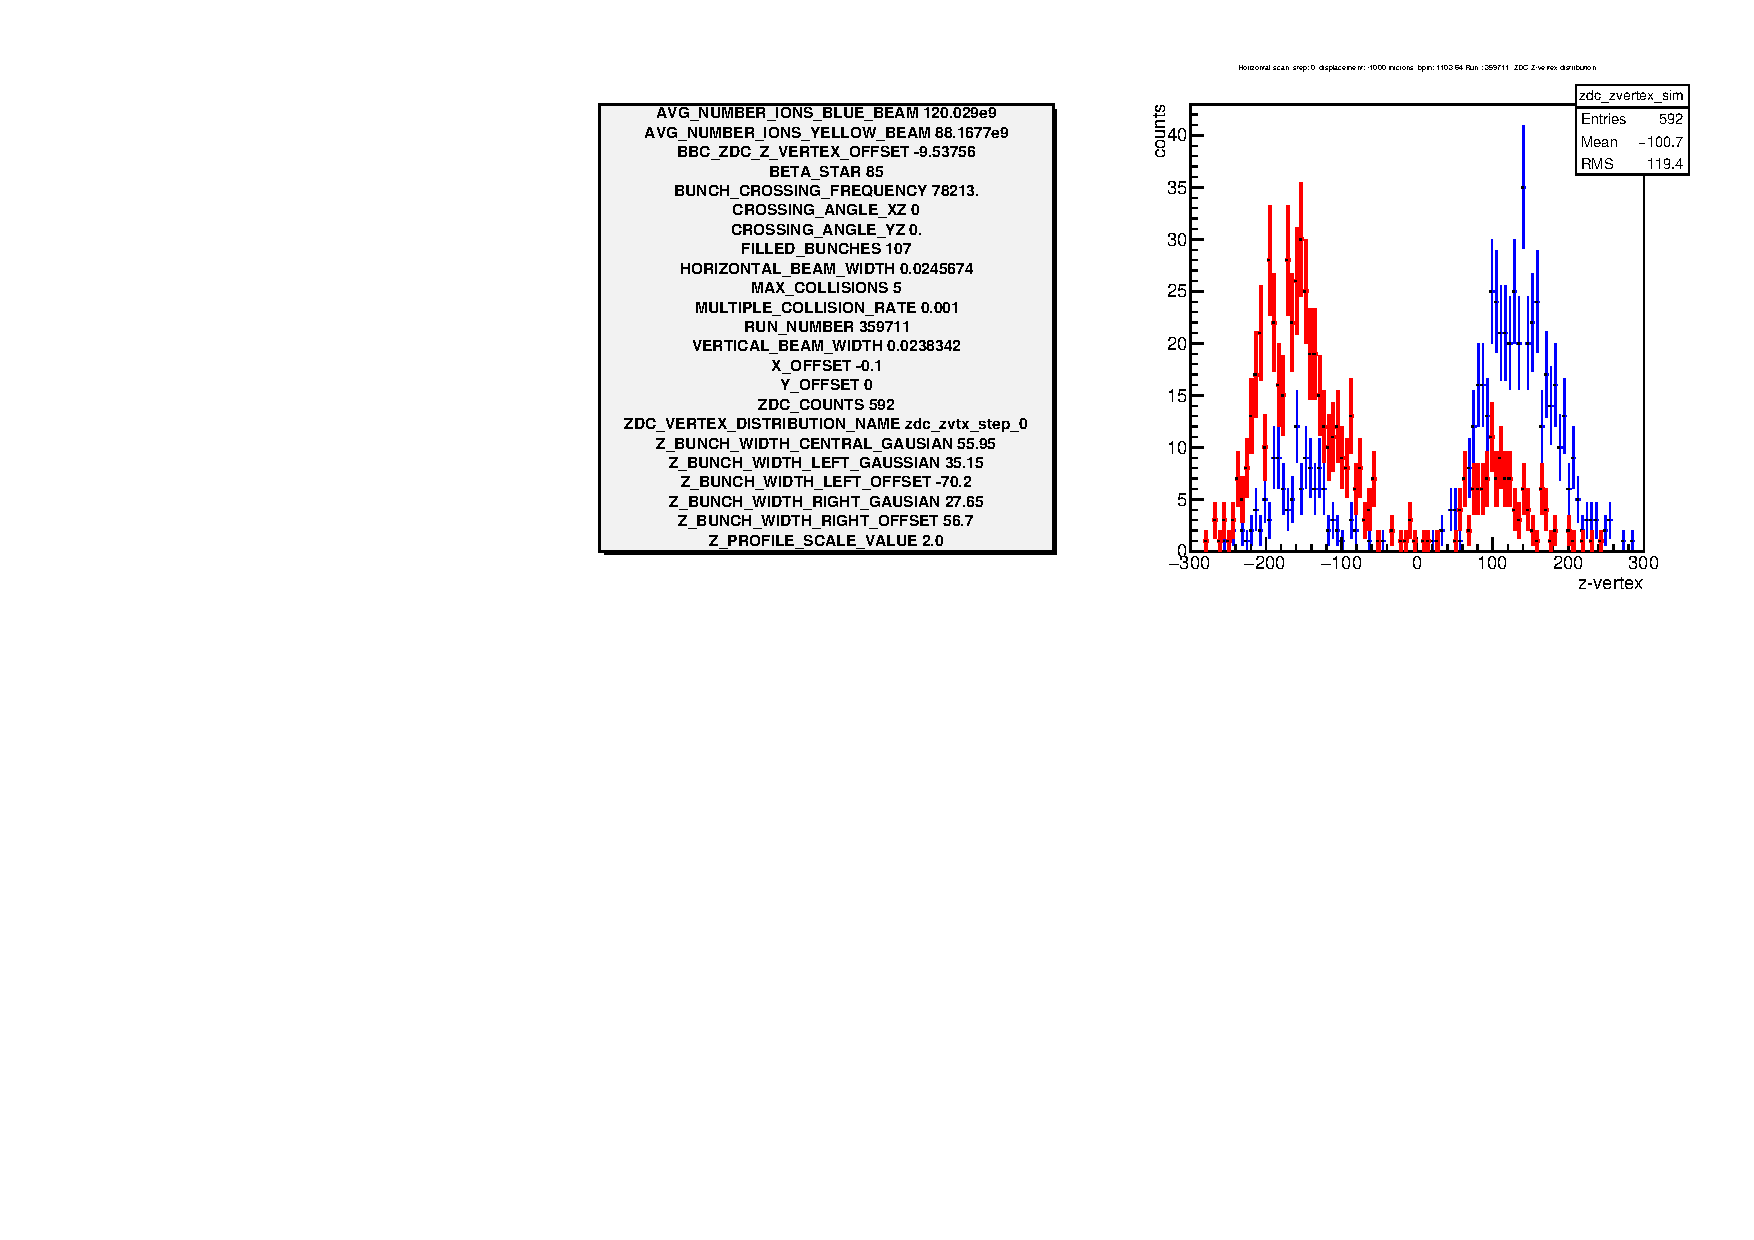
\includegraphics[width=0.75\linewidth]{../ZBunchInSimulation/figs/real_wcm_prof_zvertex_compare_hscan_pos_1000_359711_zero_xing.pdf}
\end{center}
\caption{ Using the "real" Z Profile for colliding bunches, assuming no crossing
angle}
\label{fig:real_wcm_prof_zvertex_compare_hscan_pos_1000_359711_zero_xing}
\end{figure}
\end{frame}

\subsection{Discussion of Results, Next Steps}

\begin{frame}{Discussion}
\begin{itemize}
\item Why flip bunches? Because maybe I have the direction of travel incorrect!
\item We can see from the comparison of using a simple (incorrect) model for the
	bunch z-profile can drastically alter the results of the simulation
\item We can see that the crossing angle is perhaps not well nailed down.
\item The problem now is that using this new bunch model has increased
	simulation time from 35 seconds to 20 minutes.
\item Reducing the run time of the simulation will drastically speed up
	progress.
\item The Z-Profile of the bunch is extremely important to getting the right
	answer - and incorrect profile can make affects (such as a crossing
	angle) appear to happen when there is none.
\item After substituting in a different z-profile, I have to triple-check the
	simulation code, to make sure its doing the right thing.
\end{itemize}
\end{frame}

\begin{frame}{Possible Optimization?}
The simulation takes 20 minutes, which is due entirely to how TGraph::Eval
works. It does the following:

\begin{itemize}
\item Performs a sort on three separate arrays representing the data in the
	TGraph (if specified) 
\item Performs a linear search through the TGraph internal arrays for the
	nearest x-value 
\item Performs a spline-interpolation to obtain the an approximate y-value
\end{itemize}
The typical WCM profile consists of 2100 points, and as seen in
Figure~\ref{fig:bwcm_zprofile_359711_density}, this corresponds to a z-vertex
resolution of 1.4 cm.
\end{frame}

\begin{frame}{Possible Optimization?}
\begin{itemize}
\item The features of the WCM distriubtion in
	~\ref{fig:bwcm_zprofile_359711_density} seem to have a characterstic
	resoltution scale that is larger than 1.4 cm.
\item The main issue is that we calculate coordinate transformations based on
	the crossing angle, which is a parameter we wish to vary over the
	simulations, rending precalculation impossible - \textbf{i.e. we cannot
	escape interpolation when using data directly.}
\item My guess is the linear search impacts run-time the most, followed by
	spline approximation.
\item Might also go faster if we made WCM data more coarsely binned
\item Linear search: $\mathcal{O}n \rightarrow 2100$
\item Binary search: $\mathcal{O}log(n) \rightarrow 3.2$ 
\item Probably pretty big improvement
\item Implement density as an STL object to take advantage of faster searching
	algorithms.
\end{itemize}
\end{frame}

\section{Conclusions}

\begin{frame} {Conclusions}
\begin{itemize}
\item "Real" bunch profile is available and simulation is running
\item Heavy optimization needed - and may ultimately speed things up quite a lot
\item Need to re-evaluate the rest of the luminosity calculation loop, the
transformations to $x$, $y$, $z$, $\rho(x,y,z\pm ct)$ and $\sigma_{x,y}$ do not
seem totally consistent with literature, need to check that I'm not missing a
simplification or something.
\end{itemize}
\end{frame}

\begin{frame}{The End!}
Thanks for your attention and questions!
\end{frame}
